% !TeX document-id = {9ccc6fb7-c5f4-4308-9c17-4c226ad62230}
%%%%%%
%
% $Autor: Alpizar, Kumari, JK $
% $Datum: 2023-01-31 11:59:00Z $
% $Version: 1.0.0 $
%
%
% !TeX encoding = utf8
% !TeX root = Rename
% !TeX TXS-program:bibliography = txs:///biber
%
%%%%%%

%\usepackage{graphicx} %package to manage images
\graphicspath{ {./images/} }

\chapter{Domain Knowledge}\label{DomainKnowledge}
The main scope of our project is to incorporate the ESP32 Cam device to convert the analog readings in the water and electricity meter into a digital one. The ESP32 cam will detect the last numerical digit from the electricity meter and convert it into a digital one.
\section{Tiny ML}
TinyML is a field of study which lies in the Machine Learning, Deep Learning and Embedded Systems which explores the various types of models that can run on relatively compact and energy efficient devices such as microcontrollers.\autocite{Arun:2020} The TinyML is capable of running both machine learning as well as deep learning models in resource constrained devices which are of small size and consumes low power of few milliwatt or lesser. Due to the limited memory available on these devices, large machine learning models are optimised and reduced in size.\\

The TinyML provides a number of advantages over the traditional machine learning like low-latency, low bandwidth and low power consumption while still having the functionality to be transformed into a large machine learning model. It also eliminates the privacy limitations of traditional Machine Learning as the model runs on edge devices which does not store your data in any servers.\autocite{Arun:2020}

\section{TensorFlow/ TensorFlow Lite/ Tensor Flow Micro}
TensorFlow is an open-source software library which was developed by Google to build and train machine learning models with deep neural networks. TensorFlow Lite is a lighter version of the TensorFlow.
TensorFlow Lite is also an open-source deep learning framework which is specifically designed for on-device computing in edge devices. TensorFlow Lite enables the developers to run their trained models on edge devices, computers and mobiles. TensorFlow Lite provides the ability to perform predictions on an already trained model.\autocite{Boesch:2022}\\
\begin{figure}  [H]
	\begin{center}
		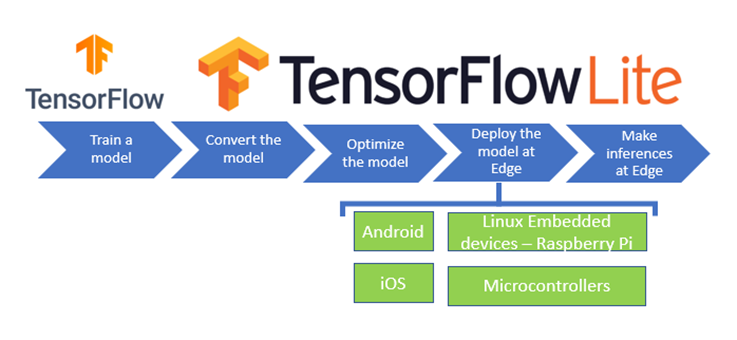
\includegraphics[width=12cm]{TFLworkflow}
		\caption{Tensor Flow Lite Workflow} 
		\label{fig:Visual Studio Code Download Options}
		\footnotesize \textbf{Reference:} \autocite{Khandelwal:2020}
	\end{center}
\end{figure}
TensorFlow Lite Microcontrollers (TFLM) is designed to run machine learning models and deep learning models on microcontrollers with only a few kilobytes of memory. TFLM tackles both the efficiency requirements imposed by embedded-system resource constrains as well as the fragmentation challenges and makes cross-platform interoperability possible. The TFLM framework adopts a unique interpreter-based approach that provides flexibility while overcoming the forementioned challenges.\autocite{David:2021}
%%%%%%%%%%%%%%%%%%%%%%%%%%%%%%%
\section{Algorithm: Convolutional Neural Network}

Convolutional Neural Network (CNN) most common use is as a type of Deep Learning model which takes in an input picture and then assign importance (biases and learnable weights) to various features that is present in the image, and can differentiate one feature from the other features. \\

The primary task of a CNN is to compress the picture into a format which is comparatively much easier to process than the full-size image. This is done while preserving crucial elements which are required for obtaining a fair prediction. The CNN enables the architecture to be competent of learning features and scalable to bigger datasets. \\ \autocite{Saha:2018}

The convolution neural network consists of three important layers which are as follows
\begin{itemize}
	\item	Convolution Layer
	\item	Pooling Layer
	\item	Fully-connected Layer
\end{itemize}
	
The complexity of the CNN increases with each layer as it identifies larger portions of image. The beginning layers focuses on simple features like edges, borders and colors. With the progression of image data through the different layers of CNN, the CNN starts to identify larger shapes and elements present in the object. This stops when the CNN identifies the intended object. \autocite{Education:2020}

\begin{figure}  [H]
	\begin{center}
		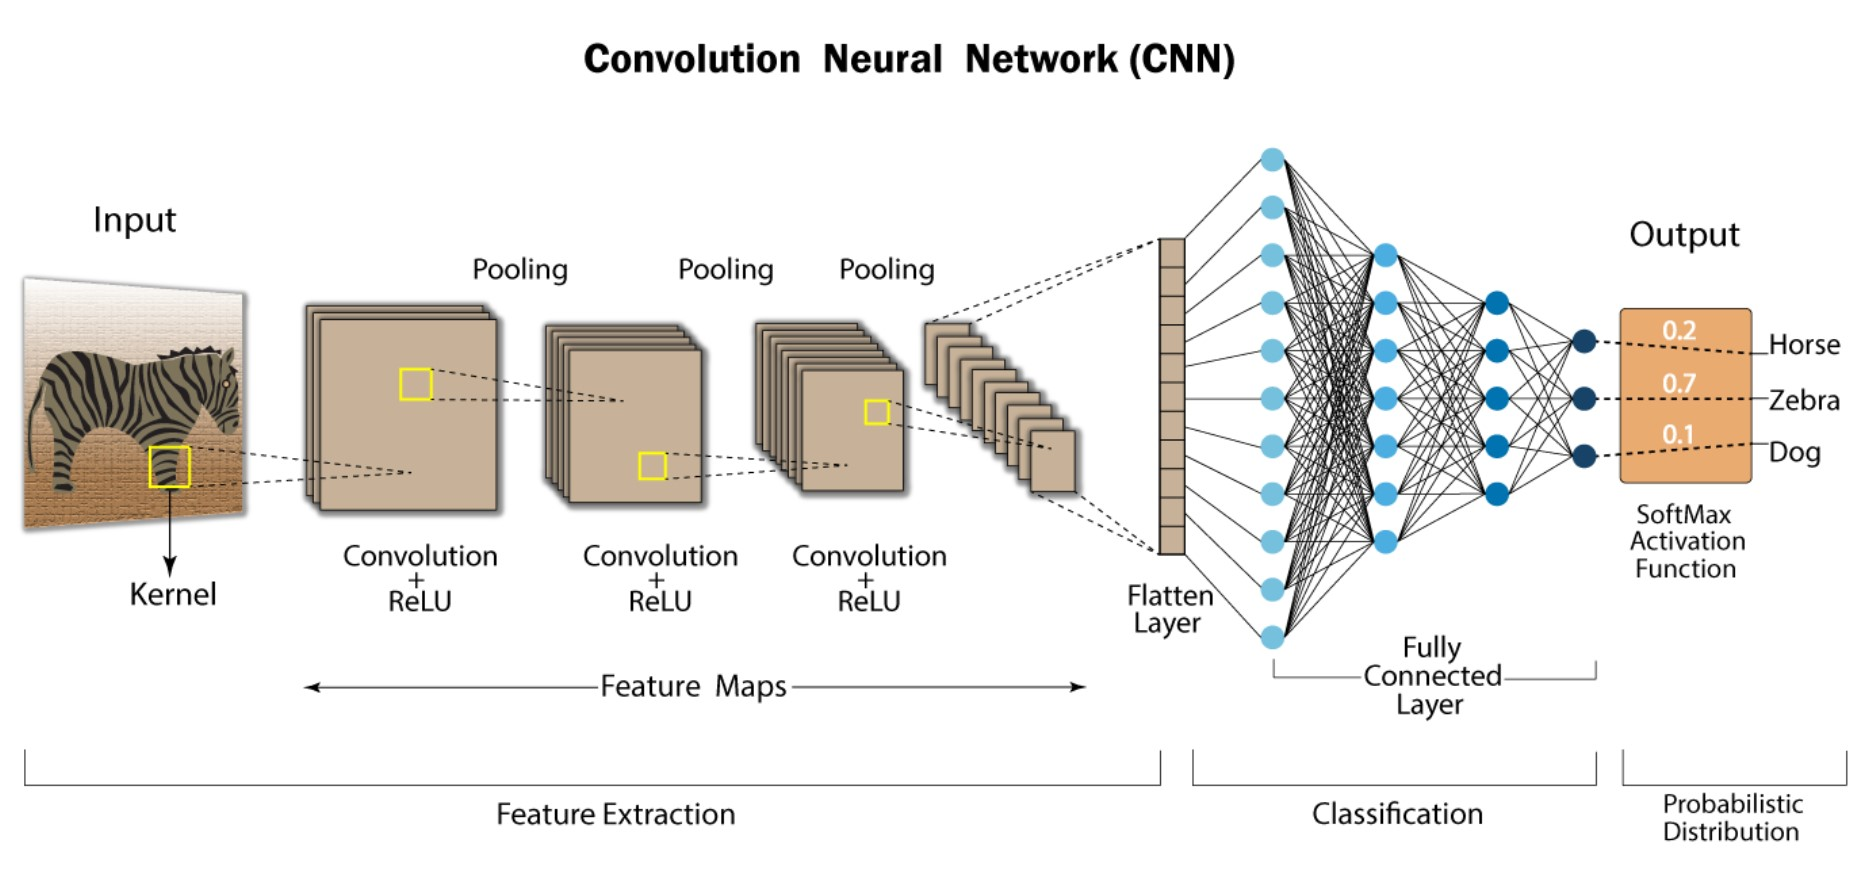
\includegraphics[width=16cm]{cnn}
		\caption{A CNN sequence to classify handwritten digits} 
		\label{fig:A CNN sequence to classify handwritten digits}
		\footnotesize \textbf{Reference:} \autocite{KE:2022}
	\end{center}
\end{figure}



The major part of the computation takes place at this layer. The components of the convolution layer are the input data, filters and feature map. The filter is also known as kernel or a feature detector. The feature detector moves through the recurring fields of the picture, while checking if the feature is present. This entire process is termed as convolution.\\

The Kernel is a two-dimensional array of biases or weights, which represents a part of the picture. The kernel can be of different sizes. This size of the kernel influences the size of receptive field. A dot product is computed between the kernel and the filter. This value of the dot product is then provided into an output array. Then the kernel moves to the next stride, this process is repeated until the kernel moves across the full picture. The final output is termed as a convolved feature or a feature map. The initial feature map only captures Low-Level information like the colour gradient and edges. The progressing feature maps captures high-level information which results in the network that helps classification of individual features present in the image. \autocite{Education:2020}

\subsection{Pooling Layer}

Pooling conducts a dimensionality reduction of the feature map. This is done by reducing the number of input parameters. Here the CNN retains the important features of the map which is required for the classification. This process is termed as down sampling.\\

In the pooling operation a filter without any weights is used to sweep across the whole input. Here an aggregation function is applied to the values of the receptive field by the kernel. The values of the aggregation function are used to populate the output array. \autocite{Education:2020}

\begin{itemize}
	\item \textbf{Max Pooling}:	As the kernel is swept through the input, the kernel identifies the pixel with the highest value and transfers it into the output array. This helps in retaining the most important features present in the feature map.
	\item \textbf{Average Pooling}:	As the kernel is swept through the input, it computes the average value of the receptive field and transfers it into the output array.
\end{itemize}

\begin{figure}  [H]
	\begin{center}
		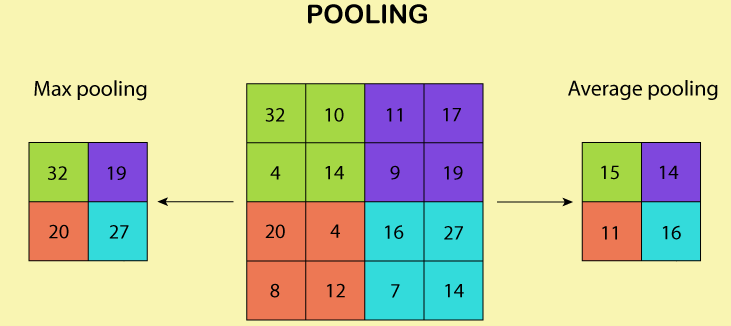
\includegraphics[width=14cm]{PoolingLayer}
		\caption{Pooling Layer in CNN} 
		\label{Pooling Layer in CNN}
		\footnotesize \textbf{Reference:} \autocite{KE:2022}
	\end{center}
\end{figure}

Pooling has benefits such as, limiting the risk of overfitting, size reduction, noise suppression and reduction in complexity of the feature map. These result in improved efficiency of the feature map.\\

\subsection{Fully-Connected Layer}
The fully-connected layer is the final layer of the CNN. Here each node of the output layer directly connects to a node of the previous layer. The classification process carried out in this layer based upon the previous layers and their appropriate filters. A Soft-Max function assigns decimal probabilities from 0 to 1 based on the appropriate classification of the inputs. \autocite{Education:2020}

\subsection{CNN Example with code}
In the following section, the required steps to train a \ac{cnn}, will be covered. There are six large sections of the code that need to be taken into account, each one of them with its own characteristics and functions. Also, the inputs and output from each code section needs to be taken into account as a priority to understand the codes functionality. \\

The main sections to create and train the \ac{cnn} are the following:  
\begin{enumerate}
	\item Preparation (loading the libraries and settings).
	\item Loading the training images.
	\item Generate training data and test data.
	\item Definition and structure of the network.
	\item Train the model.
	\item Storing the neural network.
\end{enumerate}

Now with this sections clear, it is time to jump into the coding implementation. For this it is provided the following example, including comments thru out the different code lines to better understand the purpose: 

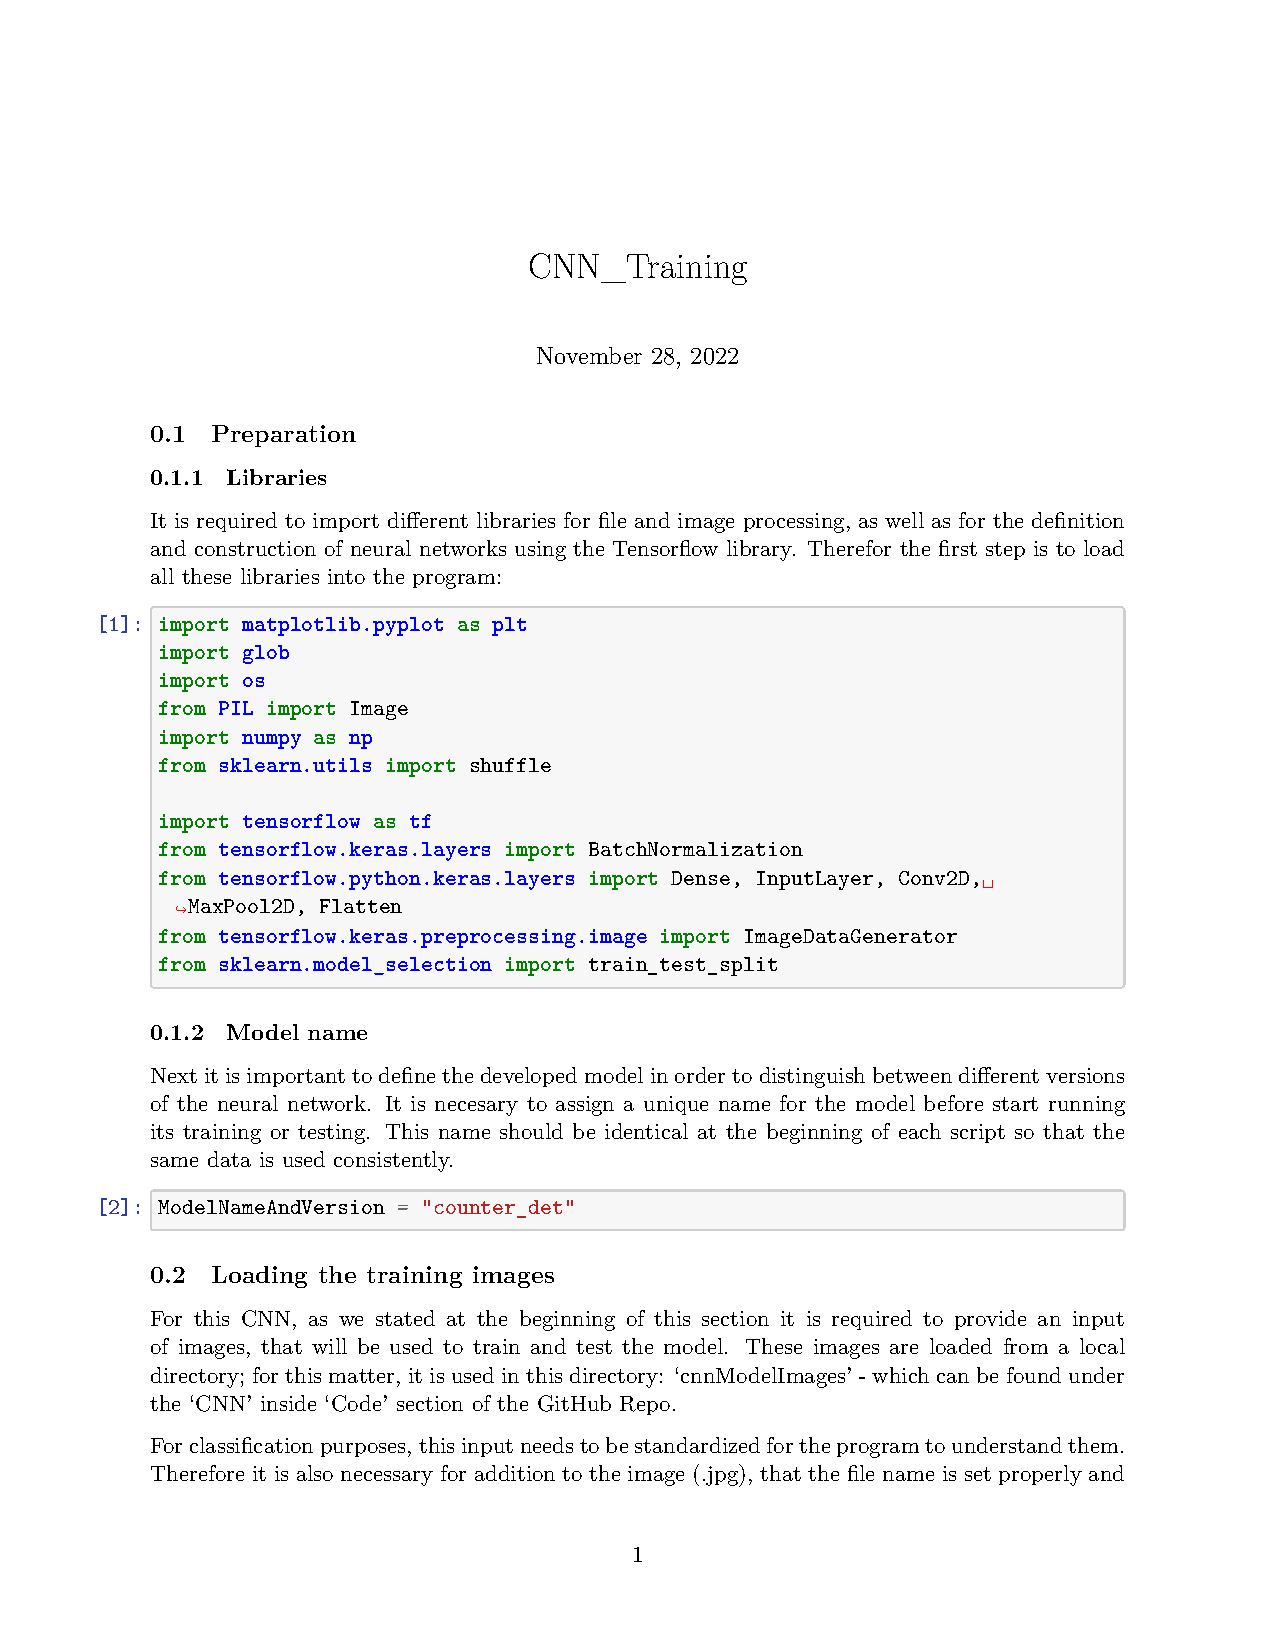
\includepdf[pages={-}]{CNNTraining.pdf}

\autocite{Muller:2020}

%%%%%%%%%%%%%%%%%%%%%%%%%%%%%%%
\section{ESP32-CAM}\label{ESP32description}
The ESP32-CAM is a low-cost full-featured microcontroller with an ESP32-S development board along with an onboard camera module and micro-SD card port. In addition, this board has integrated WiFi and Bluetooth Low Energy (BLE), which allows it to transfer data wirelessly when required.\\

ESP32-CAM is readily available in different HW Distributors online with costs ranging from around 10 Euros to 20 Euros, depending on other additional gadgets included, such as Development Board, Serial Converter, and others required for larger scale projects.\\

The small form factor, availability and economic feasibility of the ESP32 make it a perfect solution for various IoT applications such as wireless monitoring, QR code identification, image tracking, image recognition, smart home devices, industrial wireless control and other applications.\\

\subsection{Components in ESP32CAM Development Board}
The ESP32-CAM development board has the following nine components:
\begin{figure}  [H]
	\begin{center}
		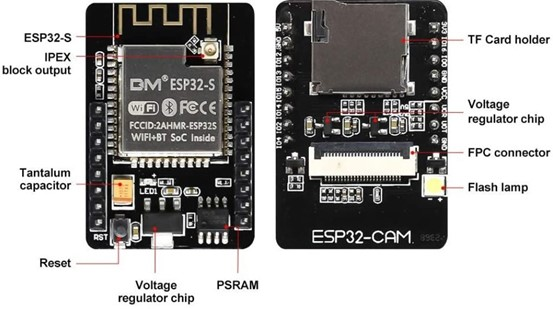
\includegraphics[width=12cm]{ESP32components}
		\caption{Components in ESP32-CAM} 
		\label{fig:Components in ESP32 Cam}
		\footnotesize \textbf{Reference:} \autocite{Lab:2021}
	\end{center}
\end{figure}

\begin{enumerate}
	\item \textbf{ESP32-S Chip}: This is the main module which houses dual core high-performance 32-bit LX6 CPUs. It computes all the processing and functioning. This supports Wireless Fidelity (Wi-Fi) and Bluetooth 4.2\\
	
	\item \textbf{IPEX block output}: The IPEX acts a connector to Global System for Mobile communication (GSM) antennas to transmit signals.\\
	
	\item \textbf{Tantalum capacitor}: Tantalum capacitor is used to provide power supply filtering for fine signal quality.\\
	
	\item \textbf{Reset button}: The reset button restarts the code that is executed on the module when pressed.\\
	
	\item \textbf{Voltage regulator chip}: The voltage regulator chip is used to regulate the voltage to 3.3 volts. This ensures that the module maintains a constant output voltage despite the fluctuations in the input power supply.\\
	
	\item \textbf{PSRAM}: This module is the Pseudo-Random-Access Memory. It consists of about 4MB memory. This enables quick processing of the instruction provided to it and assists the ESP32 camera run smoothly.\\
	
	\item \textbf{TF Card Holder}: TF Card Holder houses the Micro-SD card which stores the data in ESP32. The transmission of data between card and the ESP32-S chip takes place through the Serial Peripheral Interface.\\
	
	\item \textbf{FPC connector}: The Flexible Printed Circuit (FPC) connectors is used to mount the camera. The fine pitch of the FPC ensures the reliability of signal.\\
	
	\item \textbf{Flash Light}: The flash light module produces electric pulses which illuminates the area acts as a flash for the camera in order to take clear pictures.\\
\end{enumerate}



%%%%%%%%%%%%%%%%%%%%%%%%%%%%%%%

\subsection{ESP32-CAM Microcontroller Features}\label{ESP32specifications}

The ESP32-CAM microcontroller has the ESP32-S microprocessor module. The following are the data processing and hardware capabilities.\\
\begin{itemize}
\item Has 802.11b/g/n Wi-Fi SoC Module with a speed of 2.4 GHz
\item Has Bluetooth 4.2 with BLE
\item Has a Low-power dual-core 32-bit CPU for application processing
\item Clock speed up to 160 MHz
\item Has a summary computing power goes up to 600 DMIPS
\item Has a Built-in 520 KB SRAM plus 4 MB PSRAM
\item Supports UART, SPI, I2C, and PWM interfaces
\item Supports Wi-Fi Image Upload
\item Supports multiple sleep modes
\item Firmware Over the Air (FOTA) upgrades are possible
\item 9 General-Purpose Input/Output (GPIO) ports are available
\item Has a Built-in Flash LED
\item Support TF card
\item Has an onboard PCB antenna
\item Has embedded Free real-time operating system (FreeRTOS) and lightweight IP
\end{itemize}

\subsection{ESP32-S Microprocessor Specification}

The following are the specification of the ESP32-CAM:
\begin{itemize}
	\item SPI Flash: default 32Mbit
	\item RAM: built-in 520 KB + external 4MPSRAM
	\item Dimension: 27*40.5*4.5(±0.2)mm1.06*1.59*0.18”
	\item Bluetooth: Bluetooth 4.2 BR/EDR and BLE standards
	\item Wi-Fi: 802.11b/g/n/e/i
	\item Support Interface: UART, SPI, I2C, PWM
	\item Support TF card: maximum support 4G
	\item IO port: 9
	\item Serial Port Baud-rate: Default 115200 bps
	\item Image Output Format: JPEG( OV2640 support only ), BMP, GRAYSCALE
	\item Spectrum Range: 2412 ~2484MHz
	\item Antenna: onboard PCB antenna, gain 2dBi
	\item Transmit Power: 802.11b: 17±2 dBm (@11Mbps);
	                  802.11g: 14±2 dBm (@54Mbps);                              802.11n: 13±2 dBm (@MCS7)
	\item Receiving Sensitivity: CCK, 1 Mbps: -90dBm;
							 CCK, 11 Mbps: -85dBm; 
							 6 Mbps (1/2 BPSK): -88dBm;
							 54 Mbps (3/4 64-QAM): -70dBm;
						     MCS7 (65 Mbps, 72.2 Mbps): -67dBm
	\item Power consumption: Flash Off: 180mA@5V
						      Flash On and maximum brightness:310mA@5V             Deep-sleep: 6mA@5V                                    Moderm-sleep:20mA@5V                                  Light-sleep: 6.7mA@5V
	\item Security: WPA/WPA2/WPA2-Enterprise/WPS
	\item Power supply range: 5V
	\item Operating temperature: -20 °C ~ 85 °C
	\item Storage environment: -40 °C ~ 90 °C, < 90%RH
	\item Weight: 10g
\end{itemize}
%%%%%%%%%%%%%%%%%%%%%%%%%%%%%%%
\section{ESP32-CAM Camera Module}

\begin{figure}  [H]
	\begin{center}
		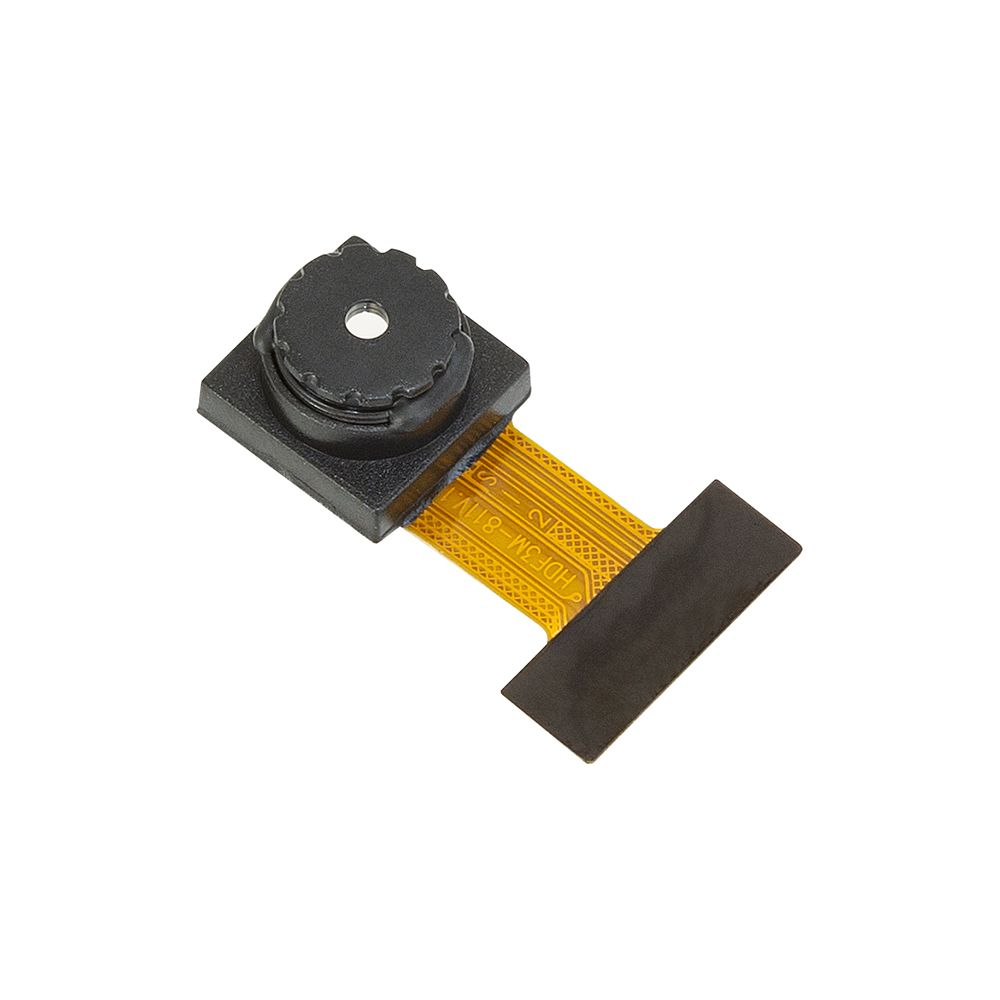
\includegraphics[width=12cm]{OV2640}
		\caption{OV2640 Camera Module} 
		\label{fig:OV2640 Camera Module}
		\footnotesize \textbf{Reference:} \autocite{}
	\end{center}                                   
\end{figure}

The ESP32 Cam uses the OV2640 camera module, which was the world’s first 1/4-inch 2 MP fully-integrated image sensor. The OV2640 image sensor has some notable features such as automatic exposure control (AEC), automatic grain control (AGC), automatic white balance (AWB), automatic band filter (ABF), and automatic black-level calibration (ABLC). One of the most beneficial features of the OV2640 is its embedded compression engine which supports most common compression formats. The image sensor also allows the user to control the image quality controls such as sharpness (edge enhancement), colour saturation, white pixel canceling, noise reduction, variable frame rate and 50/60Hz luminance detection. OV2640 image sensor has high sensitivity for low-light operations and supports formats such as Raw RGB, RGB(RGB565/555), GRB22, YUV (422/420) and YCBCr (4:2:2) formats.
\pagebreak

\begin{table}[]
	\begin{tabular}{|cc|l|}
		\hline
		\multicolumn{1}{|c|}{\textbf{Array Size}}                                                                              & \textbf{UXGA}                    & 1600 X 1200                               \\ \hline
		\multicolumn{1}{|c|}{\textbf{Power Supply}}                                                           & \textbf{Core}                    & 1.3VDC                                    \\ \cline{2-3} 
		\multicolumn{1}{|c|}{}                                                                                                 & \textbf{Analog}                  & $\sim$3.0VDC                              \\ \cline{2-3} 
		\multicolumn{1}{|c|}{}                                                                                                 & \textbf{I/O}                     & 1.7V to 3.3V                              \\ \hline
		\multicolumn{1}{|c|}{\textbf{Power Requirements}}                                                     & {\textbf{Active}} & 125 mW (for 15 fps, UXGA YUV mode         \\ \cline{3-3} 
		\multicolumn{1}{|c|}{}                                                                                                 &                                  & 140 mW (for 15 fps, UXGA compressed mode) \\ \cline{2-3} 
		\multicolumn{1}{|c|}{}                                                                                                 & \textbf{Standby}                 & 900 µA                                    \\ \hline
		\multicolumn{1}{|c|}{\textbf{Temperature Range}}                                                                       & \textbf{Stable Image}            & 0°C to 50°C                               \\ \hline
		\multicolumn{2}{|c|}{\textbf{Output Formats (8-bit)}}                                                                                    & • YUV(422/420)/YCbCr422                   \\ \cline{3-3} 
		\multicolumn{2}{|c|}{}                                                                                                                                    & • RGB565/555                              \\ \cline{3-3} 
		\multicolumn{2}{|c|}{}                                                                                                                                    & • 8-bit compressed data                   \\ \cline{3-3} 
		\multicolumn{2}{|c|}{}                                                                                                                                    & • 8-/10-bit Raw RGB data                  \\ \hline
		\multicolumn{1}{|c|}{\textbf{Lens Size}}                                                                               & \textbf{}                        & 1/4"                                      \\ \hline
		\multicolumn{1}{|c|}{\textbf{Chief Ray Angle}}                                                                         & \textbf{}                        & 25° non-linear                            \\ \hline
		\multicolumn{1}{|c|}{\textbf{\begin{tabular}[c]{@{}c@{}}Maximum Image \\ Transfer Rate\end{tabular}}} & \textbf{UXGA/SXGA}               & 15 fps                                    \\ \cline{2-3} 
		\multicolumn{1}{|c|}{}                                                                                                 & \textbf{SVGA}                    & 30 fps                                    \\ \cline{2-3} 
		\multicolumn{1}{|c|}{}                                                                                                 & \textbf{CIF}                     & 60 fps                                    \\ \hline
		\multicolumn{2}{|r|}{\textbf{Sensitivity}}                                                                                                                & 0.6 V/Lux-sec                             \\ \hline
		\multicolumn{2}{|r|}{\textbf{S/N Ratio}}                                                                                                                  & 40 dB                                     \\ \hline
		\multicolumn{2}{|r|}{\textbf{Dynamic Range}}                                                                                                              & 50 dB                                     \\ \hline
		\multicolumn{2}{|r|}{\textbf{Scan Mode}}                                                                                                                  & Progressive                               \\ \hline
		\multicolumn{2}{|r|}{\textbf{Maximum Exposure Interval}}                                                                                                  & 1247 x tROW                               \\ \hline
		\multicolumn{2}{|r|}{\textbf{Gamma Correction}}                                                                                                           & Programmable                              \\ \hline
		\multicolumn{2}{|r|}{\textbf{Pixel Size}}                                                                                                                 & 2.2 µm x 2.2 µm                           \\ \hline
		\multicolumn{2}{|r|}{\textbf{Dark Current}}                                                                                                               & 15 mV/s at 60°C                           \\ \hline
		\multicolumn{2}{|r|}{\textbf{Well Capacity}}                                                                                                              & 12 Ke                                     \\ \hline
		\multicolumn{2}{|r|}{\textbf{Fixed Pattern Noise}}                                                                                                        & \textless{}1\% of VPEAK-TO-PEAK           \\ \hline
		\multicolumn{2}{|r|}{\textbf{Image Area}}                                                                                                                 & 3590 µm x 2684 µm                         \\ \hline
		\multicolumn{2}{|r|}{\textbf{Package Dimensions}}                                                                                                         & 5725 µm x 6285 µm                         \\ \hline
	\end{tabular}
\end{table}
\begin{center}
	{OV2640 Camera Module Specification}
\end{center}
%%%%%%%%%%%%%%%%%%%%%%%%%%%%%%%


\section{Visual Studio Code}
The ac{sw} tool to be used as editor in the project development is one of the key aspects to consider, in order to set the project's background in place. There are plenty of options to consider for this matter, however taking into account the projects capabilities and constraints, there was one clear option for the implementation. \ac{vscode} is a free editor from Microsoft, which has the enormous advantage of having a plug-in specialized for all products of the manufacturer Espressif \autocite{Espressif:2022}, to be programmed and flashed.

In this section, will be presented the different stages of the implementation, from basic installation, to basic initial test on the \ac{sw} and \ac{hw} communication.

%%%%%%%%%%%%%%%%%%%%%%%%%%%%%%%
\subsection{Installation and setup}
The first thing to make sure is that everything needed to start the project with \ac{vscode} is properly installed and ready to go. Next it is going to be presented and overview to go over the entire setup process, and explain every step to get things working properly.

Even if \ac{vscode} is already installed on the machine, to give quick glance over this section is crucial, in order to make sure that the same direction is being followed before starting the project. 

Obvious to mention, but also it is clear set that if it is the first time installing \ac{vscode}, it is highly recommend completing all of the steps in this section. With no more to add. Let’s jump in!

\begin{enumerate}
	\item Download the executable file.
	\begin{itemize}
		\item You may access the file from the link bellow.
		\begin{description}
			\item[Download Link:] \url{https://code.visualstudio.com/download}
		\end{description}
	\end{itemize}
	\item Click the option Download.
		\begin{itemize}
		\item Select the option that fits the operating system of the machine where \ac{vscode} will be installed. (e.g. Windows) 
		\item \ac{vscode} version 1.73 will be used among this report.
	\end{itemize}
	\begin{figure}  [H]
		\begin{center}
			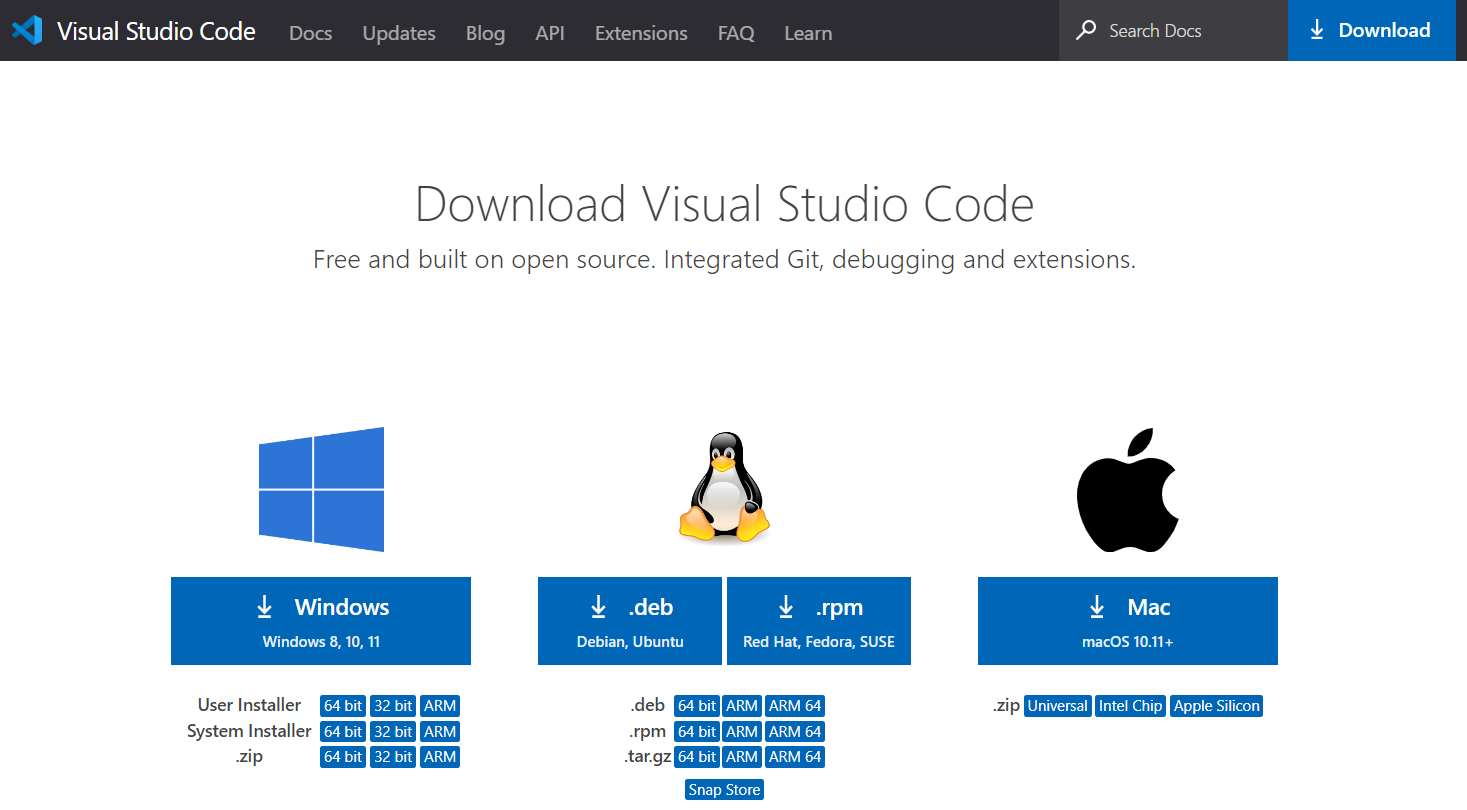
\includegraphics[width=12cm]{VSCodeDownload}
			\caption{Visual Studio Code Download Options.} 
			\label{fig:Visual Studio Code Download Options.}
			\footnotesize \textbf{Reference:} \autocite{Microsoft:2022}
		\end{center}
	\end{figure}
	\item Double click the downloaded file.
	\begin{itemize}
		\item File is stored under the name: VSCodeUserSetup-x64-1.73.0.exe
		\item Now a dialogue box appears.
		\item Select "I accept the agreement".
		\item Select "Next >".
	\end{itemize}
	\begin{figure}  [H]
		\begin{center}
			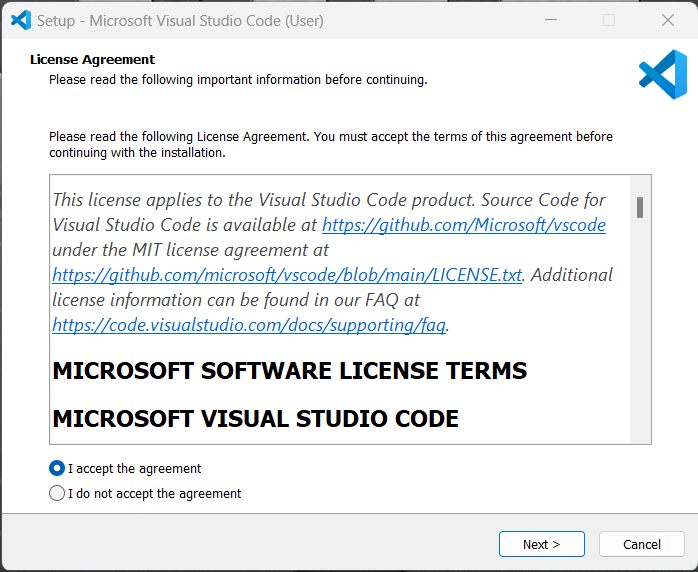
\includegraphics[width=10cm]{VSCodeInst1}
			\caption{Visual Studio Code License Agreements.} 
			\label{fig:Visual Studio Code License Agreements.}
		\end{center}
	\end{figure}
	\item Select a folder by clicking Browse or just follow the default path.
	\begin{itemize}
		\item Please note that 348.3 MB are required to be free on your device to complete the installation.
		\item Select "Next >".
	\end{itemize}
	\begin{description}
	\item[Rrecommendation: ] Leave Default path.
	\end{description}
	\begin{figure}  [H]
		\begin{center}
			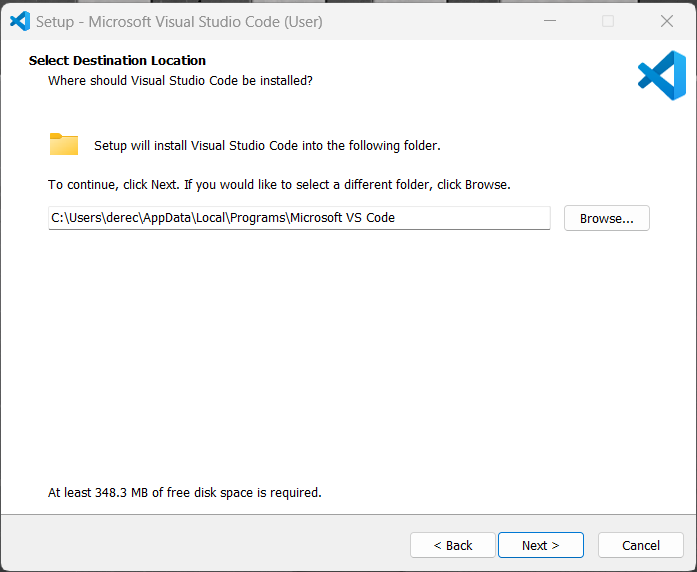
\includegraphics[width=10cm]{VSCodeInst2}
			\caption{Visual Studio Code Destination Location.} 
			\label{fig:Visual Studio Code Destination Location.}
		\end{center}
	\end{figure}
	\item Select the Start Menu Folder.
	\begin{description}
		\item[Rrecommendation: ] Leave Default path.
	\end{description}
	\begin{figure}  [H]
		\begin{center}
			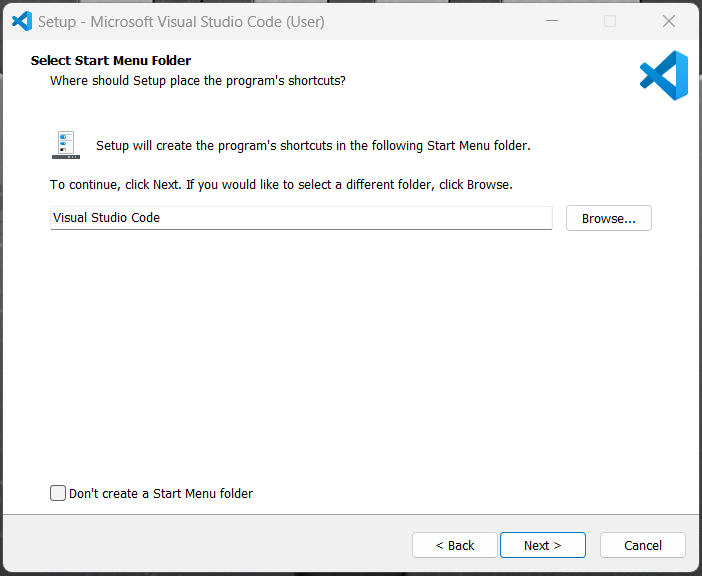
\includegraphics[width=10cm]{VSCodeInst3}
			\caption{Visual Studio Code Start Menu Folder.} 
			\label{fig:Visual Studio Code Start Menu Folder.}
		\end{center}
	\end{figure}
	\item Select Additional Tasks.
	\begin{description}
		\item[Rrecommendation: ] Leave Default path.
	\end{description}
	\begin{figure}  [H]
		\begin{center}
			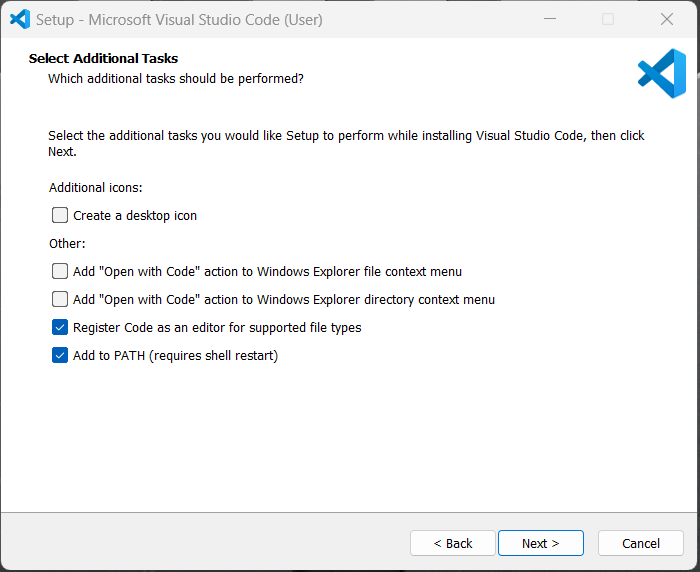
\includegraphics[width=10cm]{VSCodeInst4}
			\caption{Visual Studio Code Additional Tasks.} 
			\label{fig:Visual Studio Code Additional Tasks.}
		\end{center}
	\end{figure}
	\item Select Install.
	\begin{figure}  [H]
		\begin{center}
			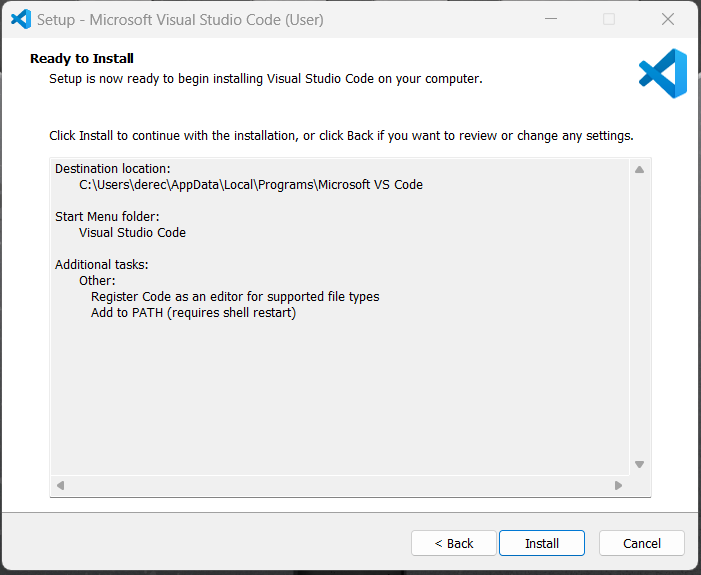
\includegraphics[width=10cm]{VSCodeInst5}
			\caption{Visual Studio Code Install.} 
			\label{fig:Visual Studio Code Install.}
		\end{center}
	\end{figure}
	\item Click Finish to exit Setup. Check in the check box to launch \ac{vscode} right now.
	\begin{figure}  [H]
		\begin{center}
			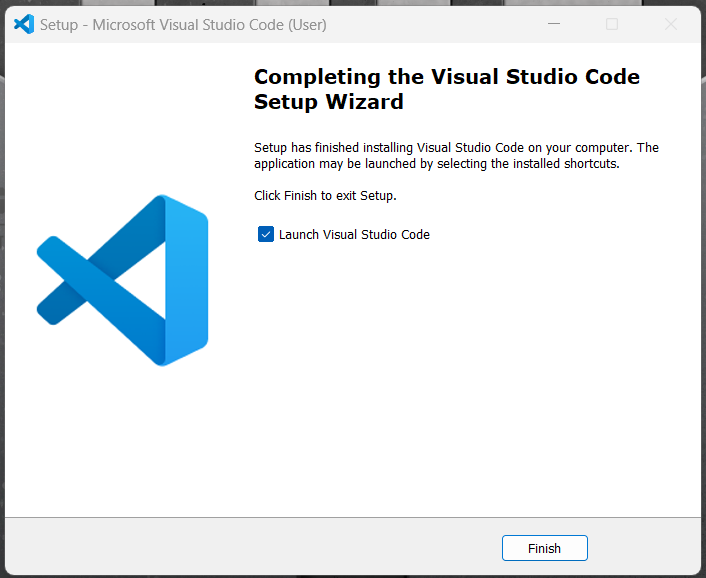
\includegraphics[width=10cm]{VSCodeInst6}
			\caption{Visual Studio Code Finished Installation.} 
			\label{fig:Visual Studio Code Finished Installation.}
		\end{center}
	\end{figure}
	\item Open Visual Studio Code and select "New File" to create a new file as a test.
	\begin{figure}  [H]
		\begin{center}
			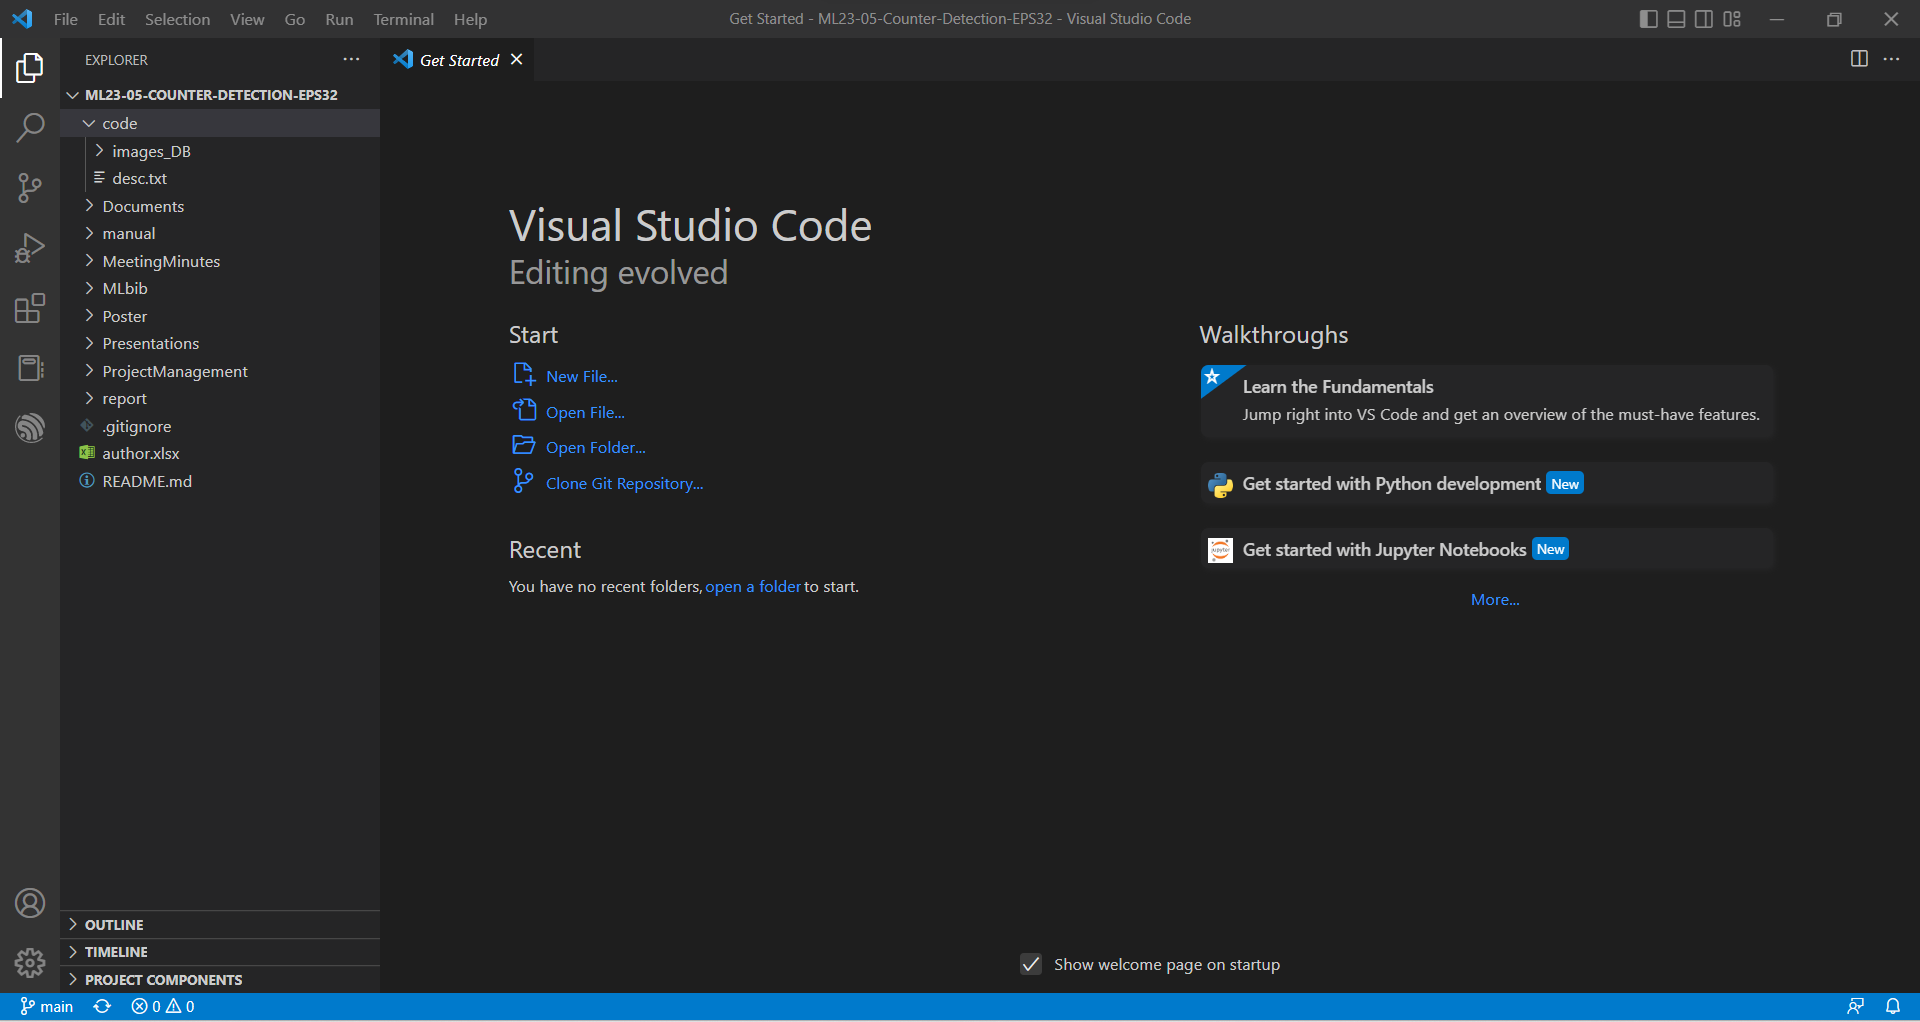
\includegraphics[width=12cm]{VSCodeInst7}
			\caption{Visual Studio Code Initial Window.} 
			\label{fig:Visual Studio Code Initial Window.}
		\end{center}
	\end{figure}
	\item For this test, select Python as development environment. 
	 \begin{itemize}
	 	\item In the new window write a basic Hello World, print function
	 	\item Use this code line: print("Hello ESP32! :)")
	\end{itemize}
	\begin{figure}  [H]
		\begin{center}
	 	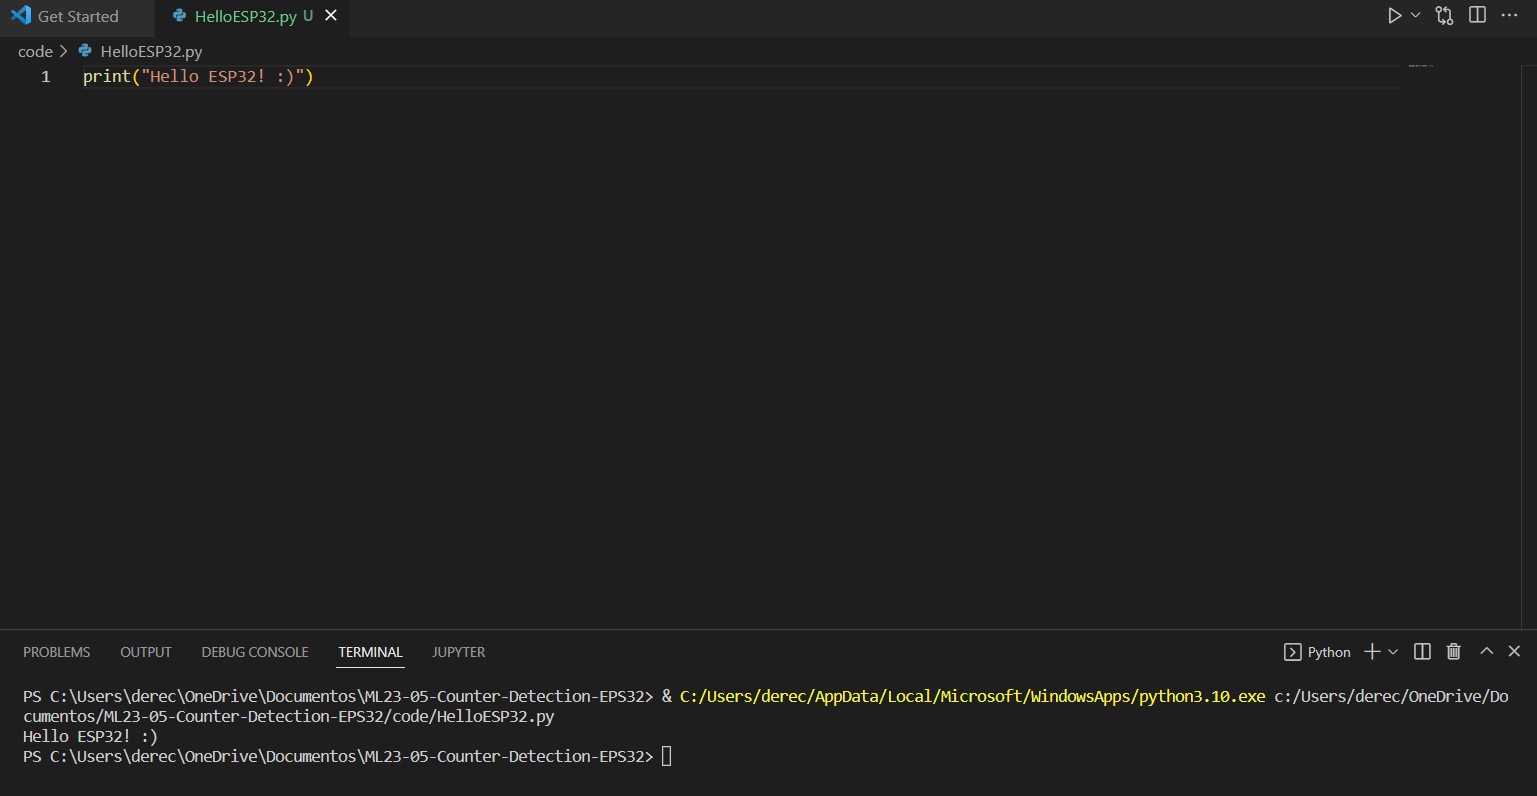
\includegraphics[width=12cm]{VSCodeInst8}
	 	\caption{Visual Studio Code "Hello ESP32 Basic Code."} 
	 	\label{fig:Visual Studio Code "Hello ESP32 Basic Code."}
	 	\end{center}
 	\end{figure}
\end{enumerate}

Congratulations. \ac{vscode} is properly installed and ready to use.

%%%%%%%%%%%%%%%%%%%%%%%%%%%%%%%
\subsection{ESP-IDF Plug-in}
ESP-IDF is the official development framework for the ESP32 family chips, in \ac{vscode}. This tool is recommended over some other options, such as Arduino IDE, because of the capability to offer more powerful applications. With this versatile plug-in it is possible to develop, build, flash, monitor and debug the code loaded in to ESP32 Devices. For this development is recommended to use version v4.4.3 (latest available), next it will be presented the setup process to get everything ready.

\begin{enumerate}
	\item Open \ac{vscode}.
	\item Open the Extensions view.
	\item Search the extension: "esp-idf"
	\item Select Install option on v1.5.1.
		\begin{figure}  [H]
		\begin{center}
			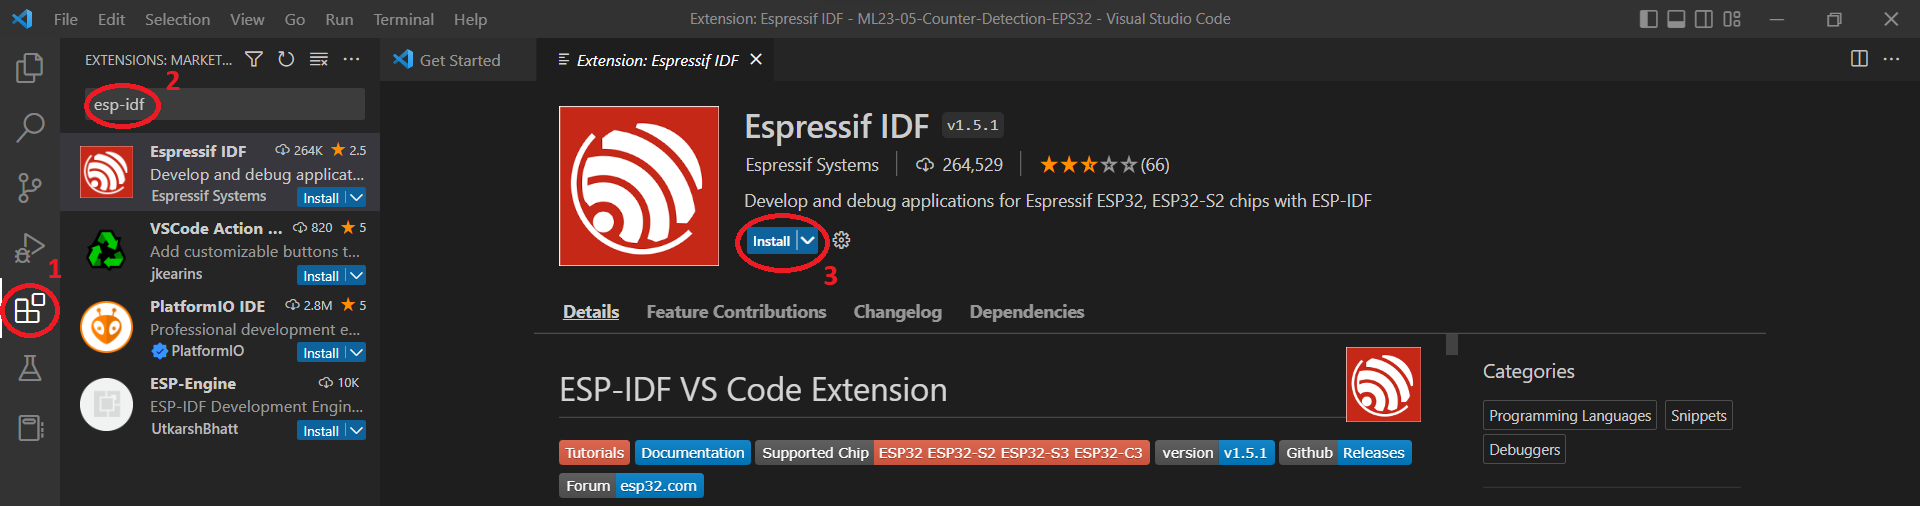
\includegraphics[width=12cm]{ESPIDFInst1}
			\caption{Visual Studio Code Install Extension "esp-df".} 
			\label{fig:Visual Studio Code Install Extension "esp-df".}
		\end{center}
	\end{figure}
	\item Select the ESP-IDF: Configure ESP-IDF extension option.
	\item Choose "Express", as the best suited option for the project.
	\item Select Install option.
	\begin{figure}  [H]
	\begin{center}
		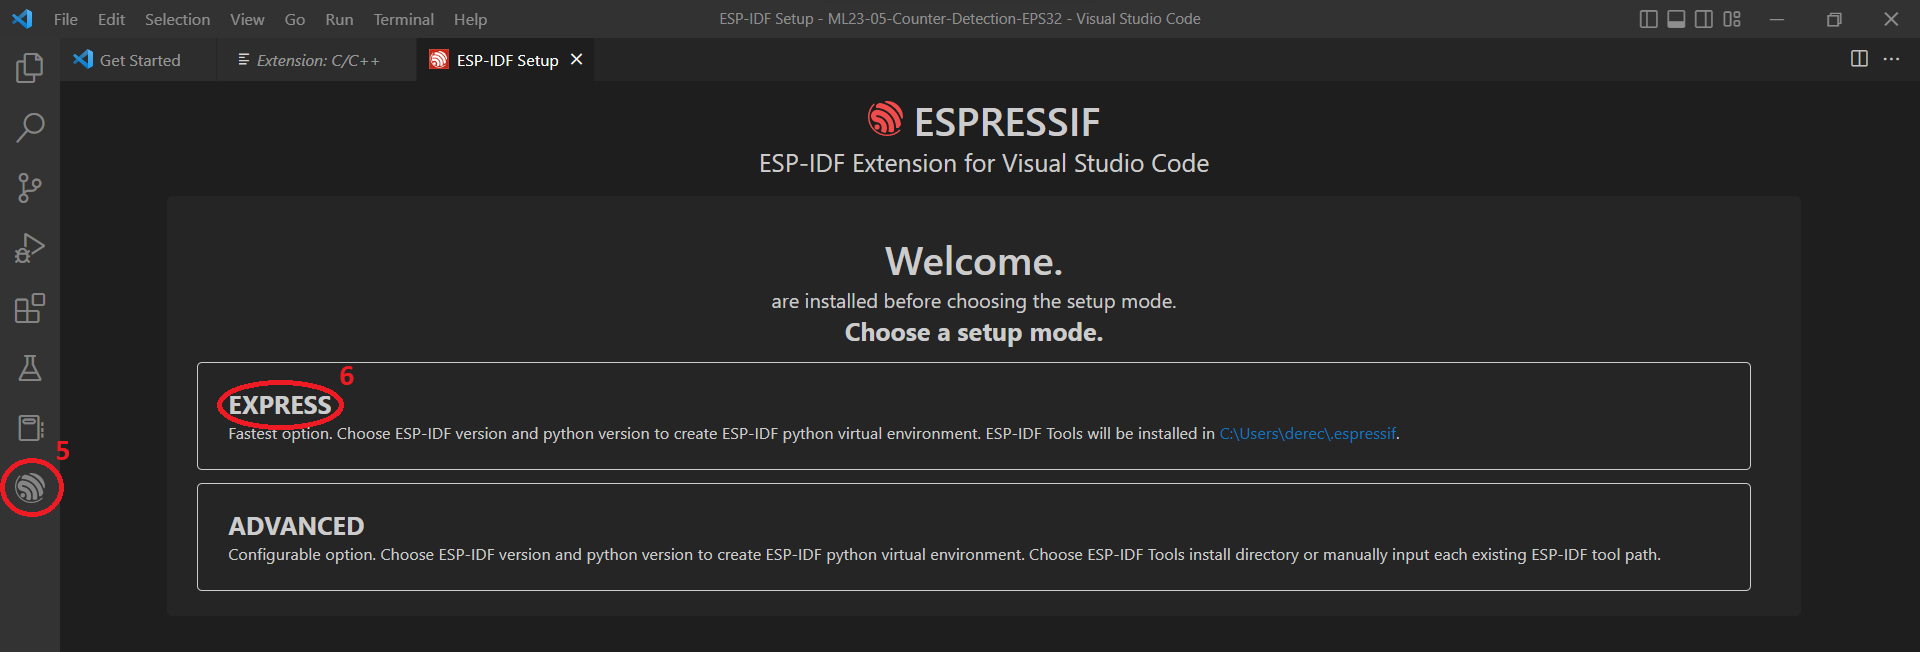
\includegraphics[width=12cm]{ESPIDFInst2}
		\caption{Configure ESP-IDF extension: Express.} 
		\label{fig:Configure ESP-IDF extension: Express.}
	\end{center}
	\end{figure}
	\item Select Download Server: "Github".	
	\item Select an ESP-IDF version to download (v4.4.3).
	\begin{figure}  [H]
	\begin{center}
		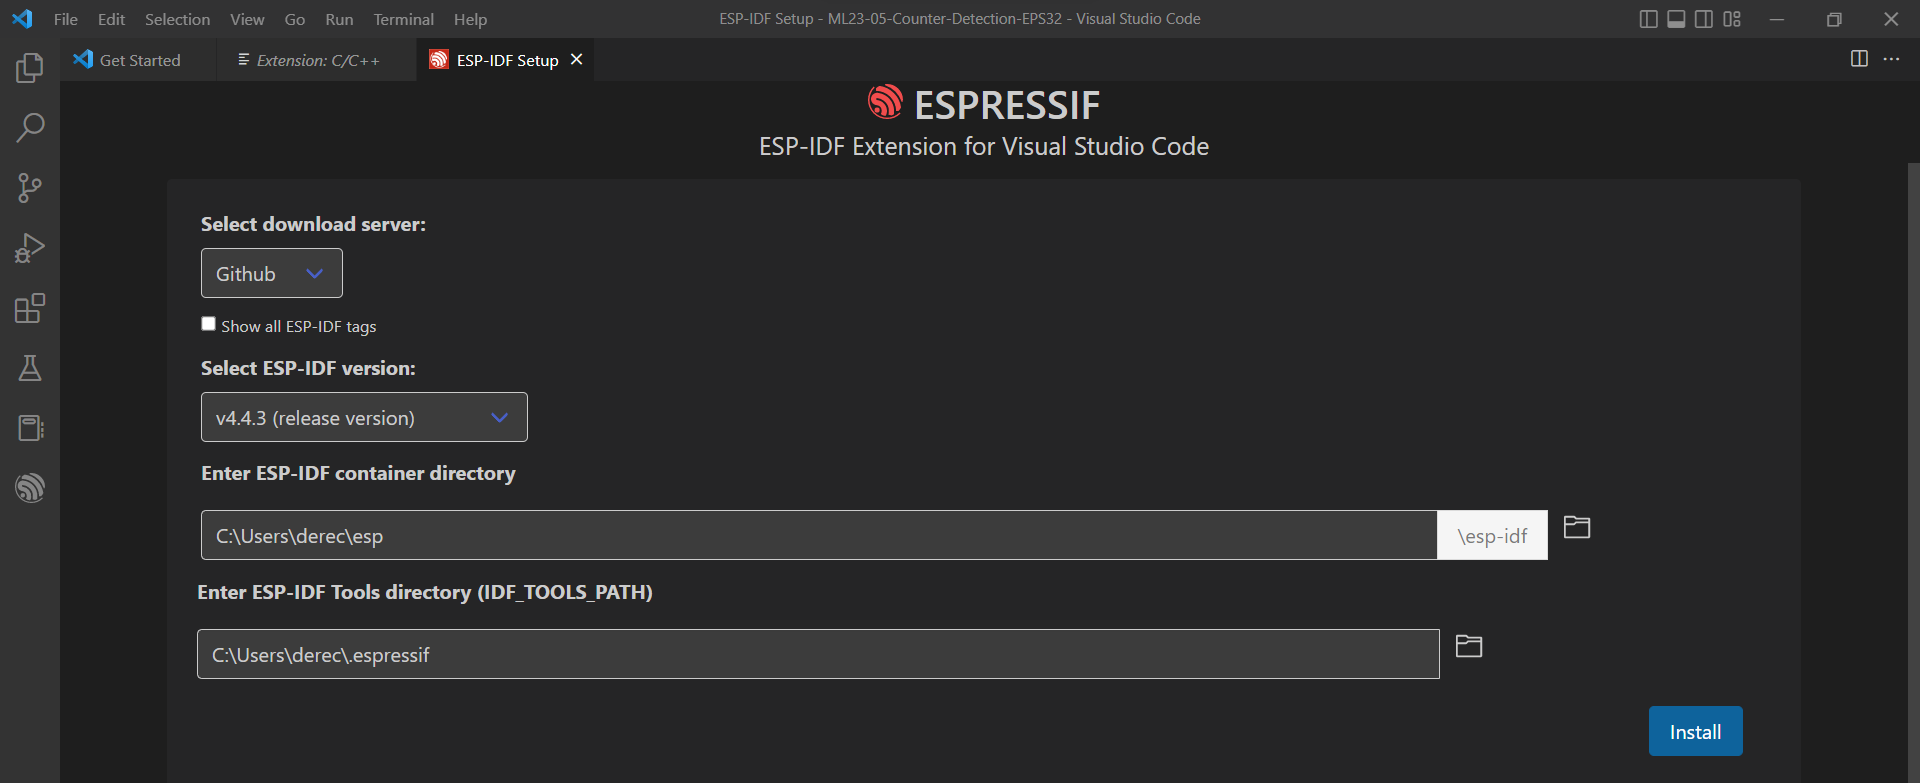
\includegraphics[width=12cm]{ESPIDFInst3}
		\caption{Download ESP-IDF version from: GitHub.} 
		\label{fig:Download ESP-IDF version from: GitHub.}
	\end{center}
	\end{figure}	
	Once the Plug-In is properly installed in \ac{vscode}, a success message will appear in the screen. \autocite{Ignacio:2022}:
		\begin{figure}  [H]
		\begin{center}
			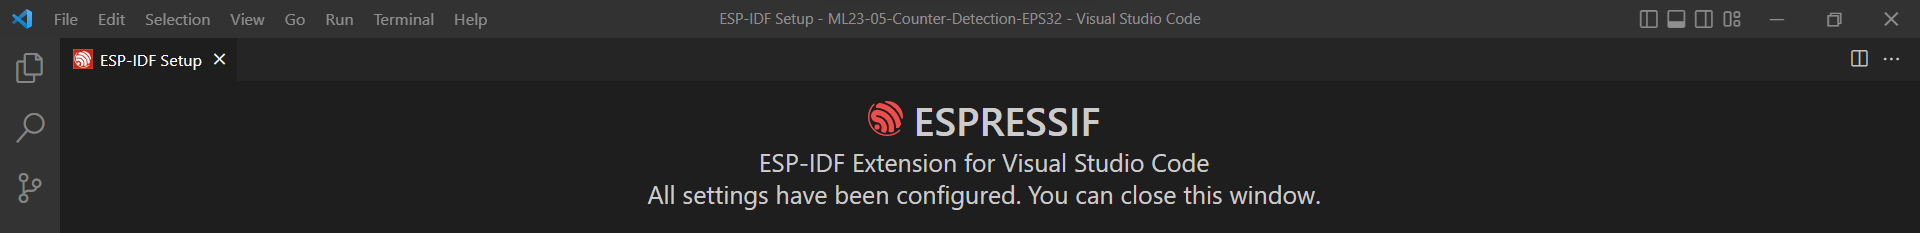
\includegraphics[width=12cm]{ESPIDFInst4}
			\caption{Successfully installed ESP-IDF.} 
			\label{fig:Successfully installed ESP-IDF.}
		\end{center}
	\end{figure}	
	It is now time to to install the ESP32-CAM drivers. \\
	The first thing to do is to clone or download and extract the repository [\href{https://github.com/espressif/esp32-camera}{ESP32 Camera GitHub project}] to the components folder of your ESP-IDF. To do this, continue with the following steps:
	\item In your Directory Navigator, go to the "ESP-IDF" pre-installed folder and look for the "components" folder. (i.e. "C:/Users/dereck/esp/esp-idf/components")
	\item Open Windows PowerShell.
	\item Run: git clone https://github.com/espressif/esp32-camera
	\begin{figure}  [H]
	\begin{center}
		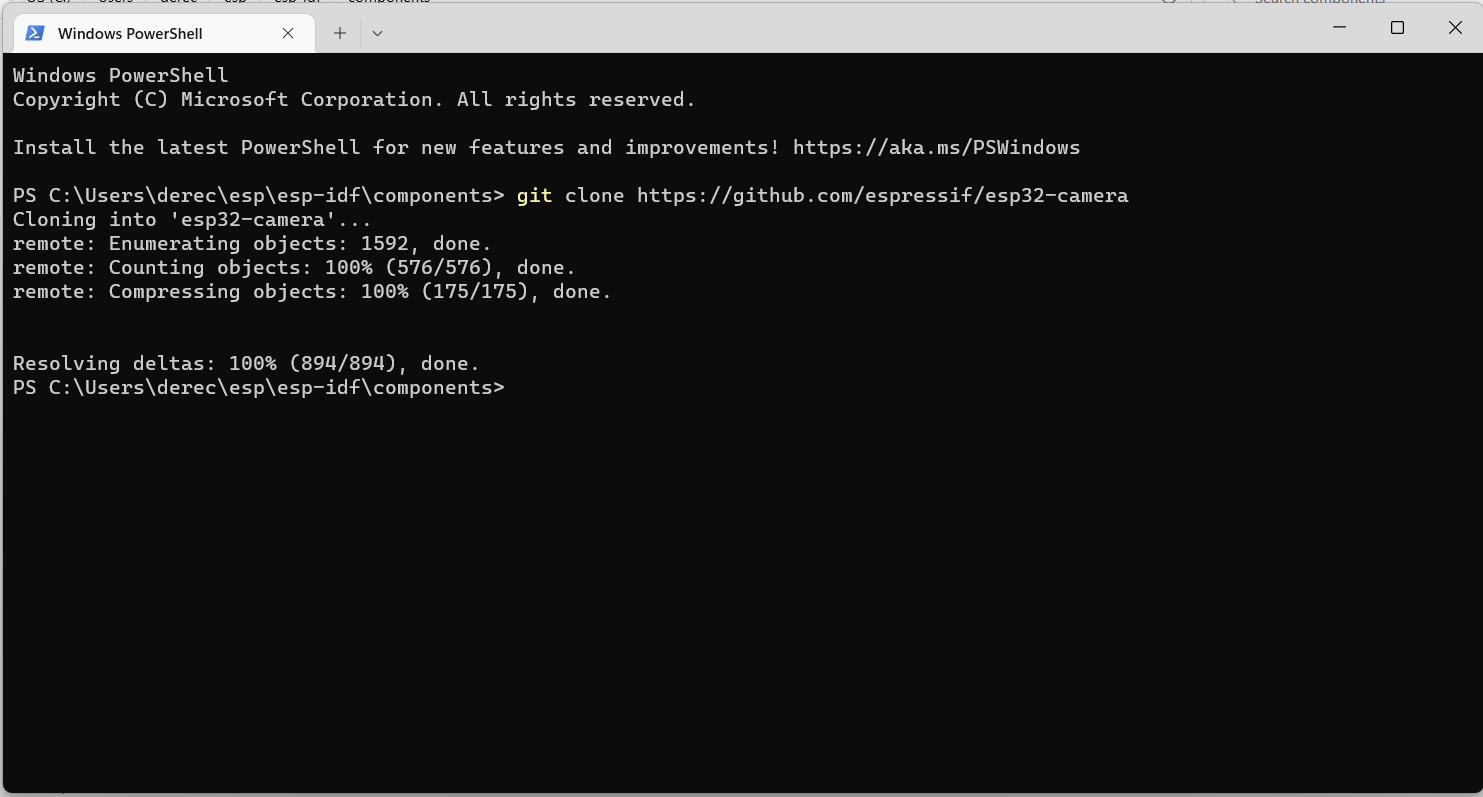
\includegraphics[width=12cm]{ESPIDFInst5}
		\caption{ESP32 Camera Clone Repository.} 
		\label{fig:ESP32 Camera Clone Repository.}
	\end{center}
	\end{figure}	
\end{enumerate}

Now all the required drivers for the ESP32-CAM are installed and ready to be used in \ac{vscode}.

%%%%%%%%%%%%%%%%%%%%%%%%%%%%%%%
\subsection{Microprocessor Test}                                                                
It is now time to test basic functionalities of the microprocessor. This will be done by loading a "Hello World" function to the \ac{hw}. For this implementation the goal is to program ESP32-S microprocessor to turn on the LED integrated in the ESP32-CAM module. To achieve this, the code will upload a basic algorithm to the ESP32-CAM module. This algorithms are part of the basic test that come along with the ESP-IDF installation. Therefore the code can be found in the installation directory of this plug-in, un de this path: "examples/get-started/blink", which is relative to the installation path (i.e. C:/Users/dereck/esp/esp-idf/examples/get-started/blink).  \\

This is the code's structure:
\begin{itemize}
	\item\textbf{Include Section: }This section includes header files that are required to run specific modules on the code. These header's location have to be defined as a path in order to avoid "building errors". This definition is done under this file: ".vscode/c\_cpp\_properties.json". In particular for the this test we need the predefined path for the ESP-IDF installation (i.e. C:/Users/dereck/esp/esp-idf).
	\item\textbf{Physical Resource Definition Section: }This section is used to indicate the code what GPIO pins must interact during the code execution. In this simple case, the conde will run only on the GPIO pin dedicated for the LED on board. This GPIO pin is defined as: "define BLINK\_GPIO 33".
	\item\textbf{Functions Section: }This section includes all the sub-functions that are going to be executed during the code. In this case we have only two functions: "configure\_led", this is used to initialize the LED condition. "blink\_led", this is used to change the LED state accordingly: HIGH or LOW. 
	\item\textbf{Main Section: }This is the principal function to be executed and this section of the code will summon accordingly the pre-defined functions. 
\end{itemize}

Once the code is ready, it has to be build, meaning that \ac{vscode} will generate a project based on the original code, and "translate" this information into a machine language code to be interpreted by the ESP32-S micro controller. This is done, on the \ac{vscode} Terminal with this command: "idf.py build". \\

Finally, Once this is ready to built code needs to be flashed or loaded to the device (ESP32-CAM). In order to do this, it is used the  \ac{vscode} Terminal with this command: "idf.py -p <PORT\_NUMBER> flash monitor". <PORT\_NUMBER> is defined by the USB resource of the computer used to connect the ESP32-CAM module. \\

This is the result of the test: 
\begin{figure}  [H]
	\begin{center}
		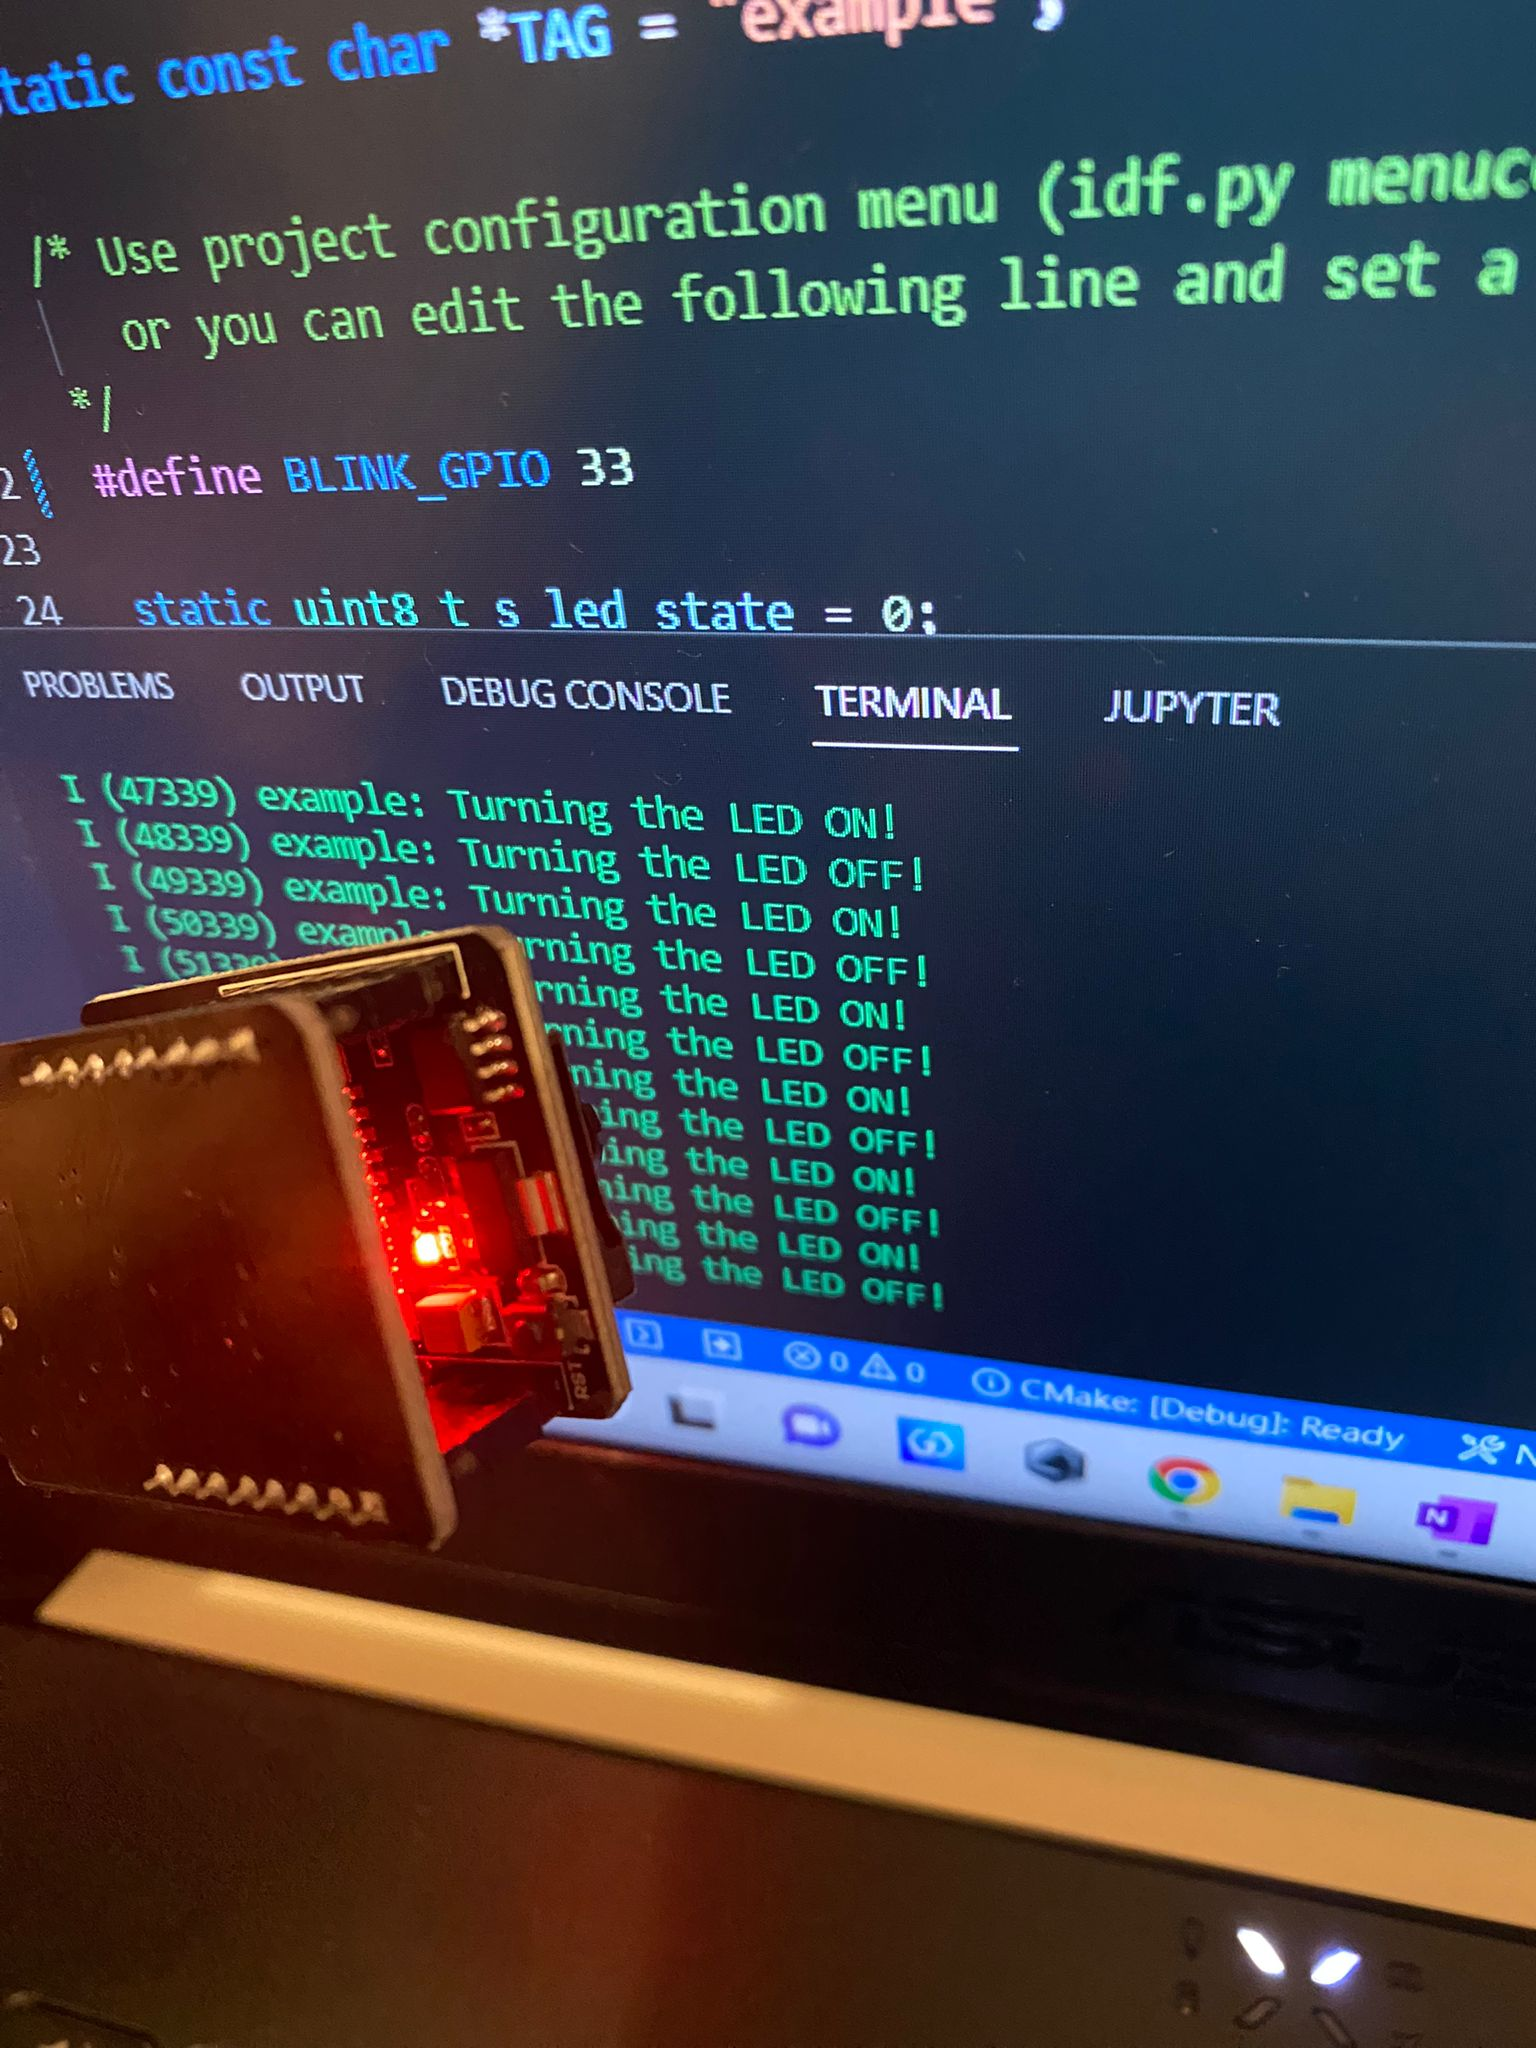
\includegraphics[width=12cm]{ESPTest1}
		\caption{Micro processor (ESP32-S) Test in ESP32-CAM.} 
		\label{fig:Micro processor (ESP32-S) Test in ESP32-CAM.}
	\end{center}
\end{figure}	

%%%%%%%%%%%%%%%%%%%%%%%%%%%%%%%
\subsection{OV2640 Camera Test}
The other key features that are key for the project to test, before the implementation are: OV2640 Camera Interaction with ESP32-CAM, and the SD-Card, proper functionality with the module. For this end, another basic "Hello World" Function is proposed. In this case the idea is to upload a code (following somehow the same strategy as the Microprocessor Test section) in this case with four major features:
\begin{enumerate}
	\item Initialize the OV2640 Camera to take pictures.
	\item Enable the camera to take a picture every 5s.
	\item Initialize the SD-Card in the ESP32-CAM to store pictures.
	\item Store the taken pictures in the SD-Card. 
\end{enumerate}

For this example, the code will be a little more complex in order to successfully perform the required functionalities. However it will be a modular code, meaning that each function will have a separate and modular implementation, making the code easy to understand and replicate. \\

This is the code's structure:
\begin{itemize}
	\item\textbf{Include Section: }Same as previous example.
	\item\textbf{Physical Resource Definition Section: }In this case it will be targeting the "CAM\_PIN" to perform the initialization and execute the capability of capturing pictures.
	\item\textbf{Camera Basic Configuration: } This is a really important section to consider, since it was not present on the previous example. It allows the micro controller to specify the characteristic under which the camera will perfom, by setting some basic parameters.
		\begin{enumerate}
			\item xclk\_freq\_hz [20000000], OV2640 camera can run under 20MHz or 10MHz.
			\item pixel\_format [GRAYSCALE], can select among these options: YUV422, GRAYSCALE, RGB565 and JPEG.
			\item jpeg\_quality [12], a value between 0 and 63 to determine the picture quality (lower number means higher quality).
		\end{enumerate}
	\item\textbf{Functions Section: }For this example the utilized functions are basically to initalize the components, "init\_camera", to initialize the camera; and "init\_sdcard, to initialize the SD-Card.
	\item\textbf{Main Section: }This is the principal function to be executed, by executing this pre loaded feature: "esp\_camera\_fb\_get" to capture picture. Then assigning a name to the picture as : "picture\#". This \# is generated by a counter, that increases after each picture. \\
\end{itemize}
	
This is the result of the test: 
\begin{figure}  [H]
	\begin{center}
		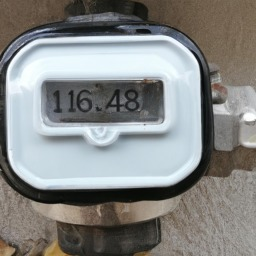
\includegraphics[width=12cm]{ESPTest2}
		\caption{Camera (OV2640) and SD-Card Test in ESP32-CAM.} 
		\label{fig:Camera (OV2640) and SD-Card Test in ESP32-CAM.}
	\end{center}
\end{figure}	
%%%%%%%%%%%%%%%%%%%%%%%%%%%%%%%



